% Template for Cogsci submission with R Markdown

% Stuff changed from original Markdown PLOS Template
\documentclass[10pt, letterpaper]{article}

\usepackage{cogsci}
\usepackage{pslatex}
\usepackage{float}
\usepackage{caption}

% amsmath package, useful for mathematical formulas
\usepackage{amsmath}

% amssymb package, useful for mathematical symbols
\usepackage{amssymb}

% hyperref package, useful for hyperlinks
\usepackage{hyperref}

% graphicx package, useful for including eps and pdf graphics
% include graphics with the command \includegraphics
\usepackage{graphicx}

% Sweave(-like)
\usepackage{fancyvrb}
\DefineVerbatimEnvironment{Sinput}{Verbatim}{fontshape=sl}
\DefineVerbatimEnvironment{Soutput}{Verbatim}{}
\DefineVerbatimEnvironment{Scode}{Verbatim}{fontshape=sl}
\newenvironment{Schunk}{}{}
\DefineVerbatimEnvironment{Code}{Verbatim}{}
\DefineVerbatimEnvironment{CodeInput}{Verbatim}{fontshape=sl}
\DefineVerbatimEnvironment{CodeOutput}{Verbatim}{}
\newenvironment{CodeChunk}{}{}

% cite package, to clean up citations in the main text. Do not remove.
\usepackage{cite}

\usepackage{color}

% Use doublespacing - comment out for single spacing
%\usepackage{setspace}
%\doublespacing


% % Text layout
% \topmargin 0.0cm
% \oddsidemargin 0.5cm
% \evensidemargin 0.5cm
% \textwidth 16cm
% \textheight 21cm

\title{Children's social referencing reflects sensitivity to graded uncertainty}


\author{{\large \bf Emily  Hembacher} \\ \texttt{ehembach@stanford.edu} \\ Department of Psychology \\ Stanford University \And {\large \bf Benjamin deMayo} \\ \texttt{bedemayo@stanford.edu} \\ Department of Psychology \\ Stanford University \And {\large \bf Michael C. Frank} \\ \texttt{mcfrank@stanford.edu} \\ Department of Psychology \\ Stanford University}

\begin{document}

\maketitle

\begin{abstract}
Recent evidence has demonstrated that children monitor epistemic
uncertainty earlier than previously believed. However, developmental
patterns across different metacognitive tasks have often been
contradictory, perhaps due to task demands involved in explicit
metacognitive reporting. The present research examined a spontaneous
behavioral reaction to uncertainty, social referencing, during a word
learning task among preschoolers. Children were asked to place a target
object in a bucket after hearing the experimenter produce a label for
the target. Referential ambiguity was manipulated through the number of
objects present and their familiarity: when there were two unfamiliar
objects and an unfamiliar label, the referent was unclear, when there
were two familiar objects, or only one novel or familiar object, the
referent was known or could be inferred. We found that children looked
up to the experimenter more often while planning and executing a
decision about which object to place in the bucket when there was
referential ambiguity. Contrary to our expectations, children looked at
the experimenter equally for ambiguous and unambiguous trials during the
labeling itself, perhaps because there was little competition for their
attention during this phase. Social referencing is a promising means of
indexing epistemic uncertainty monitoring without explicit report.

\textbf{Keywords:}
social referencing; help seeking; word learning; uncertainty.
\end{abstract}

There has been a great deal of debate over the extent to which young
children are aware of their mental states, including epistemic
uncertainty and ignorance. Although it was traditionally assumed that
preschool-aged children were either unaware of their possible ignorance
or underestimated it (Flavell, Schneider?), newer evidence shows that
preschoolers can explicitly report on their uncertainty in their
knowledge, and infants and toddlers react in ways that demonstrate
sensitivity to uncertainty. For example, preschool-aged children can use
a confidence scale to accurately report that they are less sure about
inaccurate memory (Hembacher \& Ghetti, 2014) or perceptual
discrimination decisions (Lyons \& Ghetti, Coughlin, Hembacher, Lyons \&
Ghetti).

Other research has investigated the spontaneous behaviors that infants
and toddlers engage in in response to epistemic uncertainty. For
example, Call and Carpenter (2002) had 2-year-olds choose between
several tubes to find a hidden sticker. They found that the toddlers
were more likely to peek inside a tube before choosing when they had not
seen the baiting of the tubes compared to when they had. In another
study, Goupil (year) found that 20-month-olds were more likely to seek
help by looking at their parents when they were unable to respond
accurately in a memory task.

This evidence suggests that humans are able to compute the likely
accuracy of their decisions or beliefs and act accordingly from a young
age. However, even older children have been found to fail at
metacognitive tasks that appear to rely on uncertainty monitoring. For
example, Hembacher \& Ghetti (2014) found that 3-year-olds reported
being equally confident for correct and incorrect memory decisions, and
there is protracted development of other metacognitive judgments of
performance, such as judgments of how well material has been learned,
through adolescence (refs).

Given these somewhat contradictory findings, it might be that the
ability to detect or estimate uncertainty emerges early in development,
but the ability to organize metacognitive thought processes about these
computations and translate them into strategic behavior develops more
slowly. Similar arguments have been made with regard to the distinction
between metacognitive monitoring and control; in the metacognitive
theoretical framework proposed by Nelson and Narens (1990),
metacognitive monitoring involves awareness of mental states, and
metacognitive control involves acting upon these states, for example, by
seeking new information to resolve gaps in knowledge. Many studies have
found that children's ability to report on the likely accuracy of their
knowledge or performance developmentally precedes their ability to act
on this awareness, for example, by spending more time learning difficult
compared to easy materials (refs) or refusing to answer when uncertain
(refs). Young children may react to uncertainty by hesitating or seeking
help when faced with a difficult task (refs), while older children
become increasingly able to coordinate more sophisticated learning
behaviors in response to uncertainty (refs).

Despite this progress in characterizing children's uncertainty
monitoring and related behaviors, there is still little known about the
types and sources of uncertainty that children are able to monitor, and
what spontaneous behaviors they may engage in in response to this
monitoring. These issues tie into larger questions about children's
learning. A great deal of research has focused on characterizing the
ways that young children make sense of input from their environment, for
example, when acquiring language or concepts, but there is increasing
interest in the role that children play in orchestrating the flow of
information itself (refs). Uncertainty monitoring may be a critical
factor in children's active information gathering behaviors.

One possible instantiation of this interplay may be in children's gaze
following during word learning. Gaze following allows individuals to
infer the likely referent of novel labels that occur in a speech stream,
as speakers typically gaze at their intended referent (refs). However,
at any given moment, there are multiple stimuli in the visual field that
compete for attention. In some cases, a listener may be required to
disengage from a salient or informative stimulus in order to reference a
speaker's gaze direction to resolve referential ambiguity. Thus, an
optimal system might involve referencing a speaker's gaze only when
referential ambiguity is high and gaze direction information is
necessary for disambiguation. Vaish, Demir and Baldwin (2010) found
evidence to support this possibility among 12-18-month-old infants. They
had infants sit across from an experimenter with either one or two
objects present. Infants were more likely to look up at the speaker when
she produced a novel label when there were two objects, which produced
referential ambiguity, suggesting that they were sensitive to the need
for disambiguating information.

The present research uses a similar approach to investigate
preschool-aged children's sensitivity to uncertainty based on
referential ambiguity. We aimed to replicate Vaish, Demir and Baldwin in
a new age group, and investigate the time course of social referencing
during an event in which children hear a label under ambiguous or
unambiguous conditions and are asked to select the corresponding object.
This procedure establishes social referencing as an implicit and
spontaneous measure of uncertainty monitoring, which could potentially
be used across a broad age range to investigate the development of
uncertainty monitoring and corresponding behavior.

\begin{CodeChunk}
\captionsetup{width=0.8\textwidth}\begin{figure*}[h]

{\centering 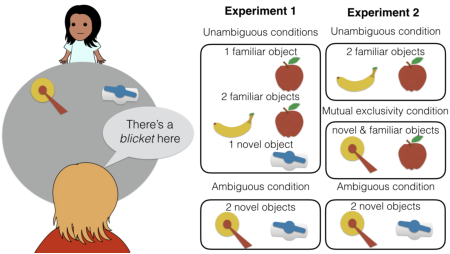
\includegraphics{figs/design-1} 

}

\caption[Study design for Experiments 1 and 2]{Study design for Experiments 1 and 2.}\label{fig:design}
\end{figure*}
\end{CodeChunk}

\section{Experiment 1}\label{experiment-1}

In Experiment 1, we examined whether children would reference a
speaker's face more often when there was referential ambiguity
associated with a label she produced. We were interested not only in
children's referencing of gaze direction during the labeling itself, but
referencing of the speaker after the labeling event while children made
a decision about which object was the intended referent. We predicted
that children would seek confirmation of the accuracy of their choice
from the speaker when they were uncertain, perhaps expecting an
emotional reaction or explicit approval, in addition to seeking gaze
direction information during labeling. We will refer to all of this
looking behavior as social referencing, as the looks could reflect
different types of information gathering.

To test this, we had children sit across from an experimenter who
labeled an object on the table between them. Across trials, there were
either one or two objects, which were either familiar or unfamiliar to
the child. We expected children to be uncertain about the label's
referent only on trials with two unfamiliar objects. After labeling an
object, the experimenter asked the child to place the named object in a
bucket. We measured the number of times the child looked up to the
experimenter's face during four discreet phases of the trial: the
labeling event (``label'' phase), the sliding of the object(s) into the
child's reach (``slide'' phase), the time before the child touched an
object once they were within reach (``planning'' phase), and the time
between touching an object and dropping it in the bucket (``response''
phase).

We predicted that children would look to the experimenter more often on
two-object novel trials compared to the other three trial types during
the labeling, planning, and response phases, which would indicate that
they recognized the need for disambiguating information. We did not
predict that children would look more for these trial types during the
slide phase, when they would likely be looking at the objects
themselves.

\subsection{Methods}\label{methods}

\subsubsection{Participants}\label{participants}

We recruited a planned sample of 80 children ages 2-5 years from the
Children's Discovery Museum in San Jose, California. The sample included
20 2-year-olds (mean age 31.71 months), 20 3-year-olds (mean age 42.65
months), 20 4-year-olds (mean age 55.85 months), and 20 5-year-olds
(mean age 65.11 months). An additional 20 children participated but were
removed from analyses because they heard English less than 75\% of the
time at home (\emph{n} = 10), because they were unable to complete at
least half of the trials in the task (\emph{n} = 4), because of parental
interference (\emph{n} = 1), or due to experimenter or technical errors
(\emph{n} = 5).

\subsubsection{Stimuli and Design}\label{stimuli-and-design}

In this task, children were presented with one or two objects, heard a
label, and were asked to put the labeled object in a bucket. Half of the
objects were selected to be familiar to children (e.g., a cow) and half
were selected to be novel (e.g., a nozzle). There were four trial types:
one-familiar, one-novel, two-familiar, and two-novel. There were three
of each trial type, for a total of twelve trials, and trial types were
presented sequentially in an order that was counterbalanced across
participants. The assignment of individual objects to trial types was
counterbalanced. On familiar trials, the familiar label for the target
object was used (e.g., ``cow''). On novel trials, a novel label was used
(e.g., ``dawnoo'').

The critical manipulation was of referential ambiguity; on one-familiar
and two-familiar trials, there was no referential ambiguity, as children
were expected to be certain about the objects and their labels.
Similarly, on one-novel trials, children were expected to be certain
about the label referent as there was only one option. However, on
two-novel trials, the referent was ambiguous, as the novel label could
apply to either novel object (Figure \ref{fig:design}).

\subsubsection{Procedure}\label{procedure}

Throughout the study, the child sat at one end of a large circular
table, and the experimenter stood at the opposite end. Each trial of the
task proceeded as follows: the experimenter placed one or two objects on
the left and/or right sides of the table, out of reach of the child so
that the child could not interact with the toys during the labeling
event. For one-object trials, the location of the object (left or right)
alternated between trials. After placing the objects, the experimenter
said ``Hey look, there's a (target) here.'' The experimenter gazed at
the center of the table rather than the object she was labeling because
we wanted to preserve the referential ambiguity throughout the trial.
The experimenter waited approximately two seconds (based on a visual
metronome placed within view) before saying, ``Can you put the (target)
in the bucket?'' She then pushed the object(s) forward within reach of
the child, and placed a plastic bucket in the center of the table, also
within reach of the child. Prior to the twelve experimental trials,
there were two training trials: a one-familiar trial and a two-familiar
trial, to acquaint the child with the procedure. A camera placed to the
side of the experimenter captured the participant's face, so that
looking behavior could be coded from video.

\subsubsection{Coding procedure}\label{coding-procedure}

Videos were coded using DataVyu software (\url{http://datavyu.org}).
First, each trial was divided into four temporal phases: a ``label''
phase, which began at the utterance of the target label and ended when
the experimenter began to slide the objects, a ``slide'' phase, which
encompassed the sliding of the objects into the child's reach, a
``planning'' phase, which began at the end of the slide and ended when
the child touched an object, and a ``response'' phase, which began when
the child touched an object and ended when the child released the object
into the bucket. After onsets and offsets of these phases had been
coded, the coder recorded the number of looks the child made to the
experimenter's face during each phase. A second coder coded the number
of looks for ¼ of the trials for each participant to establish
reliability. \emph{include reliability data here}

\subsection{Results and Discussion}\label{results-and-discussion}

\begin{CodeChunk}
\begin{figure*}[h]

{\centering 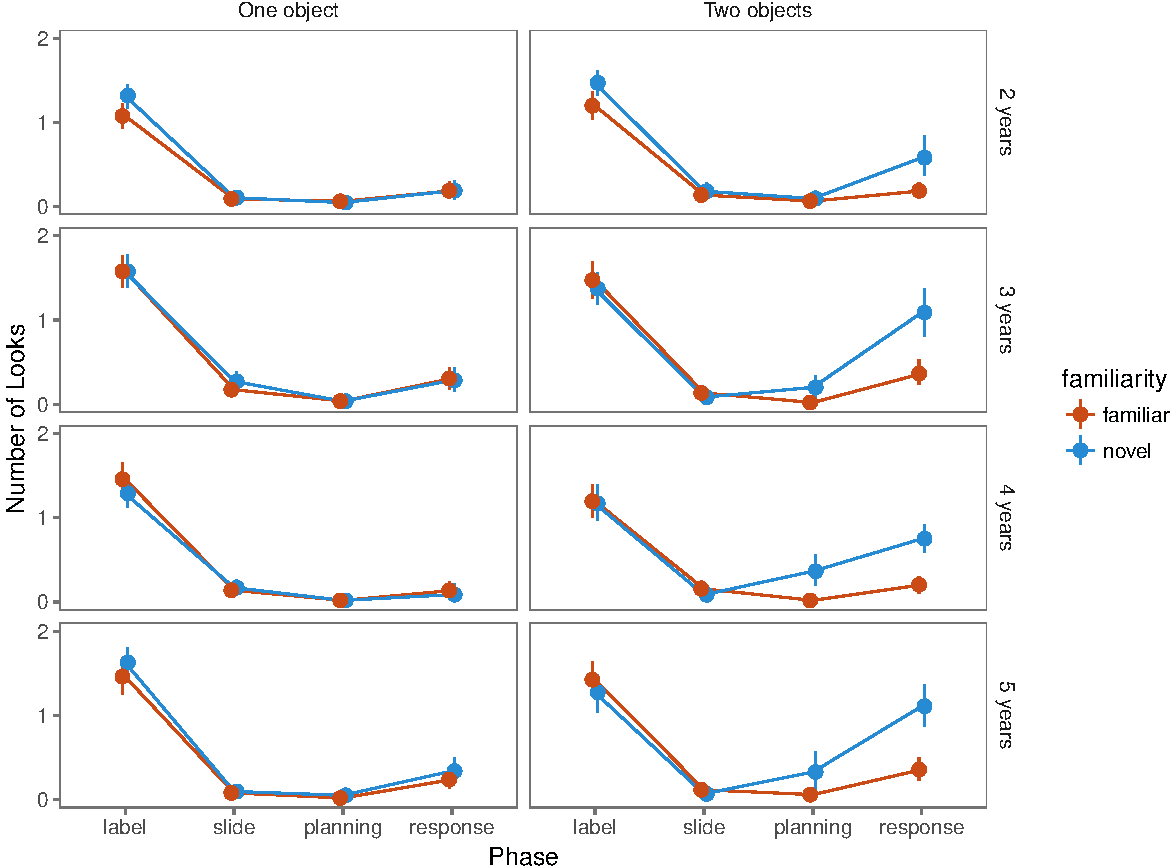
\includegraphics{figs/results_e1-1} 

}

\caption[Results of Experiment 1]{Results of Experiment 1. Number of looks to the experimenter across phases and conditions.}\label{fig:results_e1}
\end{figure*}
\end{CodeChunk}

The descriptive results of Experiment 1 are presented in Figure
\ref{fig:results_e1}. To quantify the main and interactive effects of
referential ambiguity and age on looking, we fit mixed-effects linear
regression models separately for each phase with the following
structure:
\texttt{number of looks \textasciitilde{} number of objects * familiarity * age in months + (number of objects + familiarity \textbar{} SID)}.
A single model with phase as a factor did not converge.

We did not find any main or interactive effects of number of objects,
familiarity, or age on number of looks during the label phase or the
slide phase. However, we found an interactive effect of number of
objects and familiarity during the planning (\(\beta\) = 0.21, \emph{p}
\textless{} .001) and response phases (\(\beta\) = 0.6, \emph{p}
\textless{} .001), such that 2-novel trials were associated with more
looking. There was no interaction with age in either phase.

In summary, we found that children ages 2-5 looked to the experimenter
more often when planning and executing a response under uncertainty.
This suggests that they were aware that they did not have sufficient
knowledge to answer independently, and they attempted to resolve their
uncertainty using social referencing. However, we did not find the
expected effect of referential ambiguity in the label phase. There are a
number of reasons we might have observed this null effect. One
possibility is that children failed to predict that they would need more
information until later in the trial, when they were actually faced with
planning and executing a decision. Another possibility is that
children's looking was at ceiling during the labeling phase, perhaps
because children look at someone who is speaking regardless of the need
for referential disambiguation. A third possibility is that this is an
artifact of our design, in which the experimenter gazed at the center of
the table rather than the referent of her label. Children may have
realized that the experimenter's gaze direction during labeling was not
a source of disambiguating information. Experiment 2 seeks to examine
this possibility.

\section{Experiment 2}\label{experiment-2}

Experiment 2 was designed to replicate Experiment 1 and address the
possibility that the experimenter's gaze pattern during labeling had an
effect on children's social referencing. To test this possibility, we
manipulated the experimenter's gaze behavior between participants. For
half of the sample, the experimenter gazed at the center of the table
during labeling (i.e., reproducing Experiment 1), and for the remaining
half, the experimenter looked at the object she was referring to during
labeling. In Experiment 1, we did not observe an effect of age on
looking. Thus, we restricted the current sample to 3- and 4-year-olds.
Finally, since we did not observe any difference between the
one-familiar and one-novel trials, we eliminated single-object trials,
leaving the 2-familiar and 2-novel trials. In addition to these trials,
we added 1-novel-1-familiar trials to examine children's looking
patterns when 2 objects are present and an unfamiliar label are
produced, but the label referent can be deduced through the principle of
mutual exclusivity.

\subsection{Methods}\label{methods-1}

\subsubsection{Participants}\label{participants-1}

We recruited a planned sample of 80 children ages 3-4 years from the
Children's Discovery Museum in San Jose, California. The sample included
40 3-year-olds (mean age 42.89 months) and 40 4-year-olds (mean age
53.47 months). An additional 20 children participated but were removed
from analyses because they heard English less than 75\% of the time at
home (\emph{n} = 9), because they were unable to complete at least half
of the trials in the task (\emph{n} = 7), or due to experimenter or
technical errors (\emph{n} = 4).

\subsubsection{Stimuli and Design}\label{stimuli-and-design-1}

The stimuli and design were similar to Experiment 1, except that we
eliminated 1-object trials. Instead, we included three trial types:
2-familiar (``familiar''), 2-novel (``novel''), and 1-novel-1-familiar
(``mutual exclusivity''). There were four of each trial type, totaling
twelve trials. In addition, we manipulated the experimenter's gaze
behavior between participants. For half of the participants, she looked
at the center of the table on every trial; for the remaining half, she
looked at the object she referred to on every trial.

\subsubsection{Procedure}\label{procedure-1}

The procedure was identical to Experiment 1, except that there were
three practice trials rather than two, so that children could experience
every trial type.

\subsection{Results and Discussion}\label{results-and-discussion-1}

\begin{CodeChunk}
\begin{figure*}[h]

{\centering 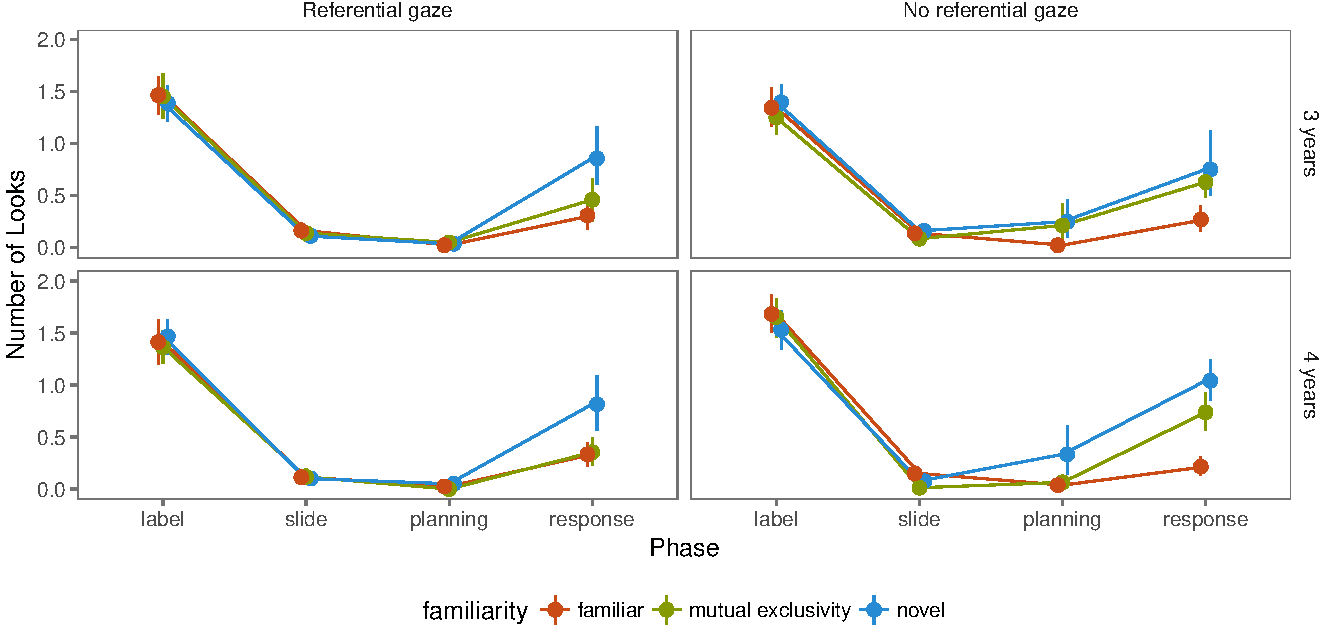
\includegraphics{figs/results_e2-1} 

}

\caption[Results of Experiment 2]{Results of Experiment 2. Number of looks to the experimenter across phases and conditions.}\label{fig:results_e2}
\end{figure*}
\end{CodeChunk}

The descriptive results of Experiment 2 are presented in Figure
\ref{fig:results_e2}. To quantify the main and interactive effects of
familiarity, number of objects, gaze behavior, and age on social
referencing, we fit a mixed-effects linear regression model with the
following structure:
\texttt{number of looks \textasciitilde{} familiarity * age in months * gaze * phase + (familiarity \textbar{} SID)}.

As in Experiment 1, there was an interaction of phase with familiarity
such that the response phase of novel trials was associated with
significantly more looks (\(\beta\) = 0.51, \emph{p} \textless{} .001).
There was a three-way interaction of familiarity, gaze, and phase, such
that the response phase of mutual exclusivity trials in the no-gaze
condition was associated with more looks (\(\beta\) = 0.39, \emph{p}
\textless{} .01). Finally, we observed a four-way interaction such that
the response phase of novel trials in the gaze condition was associated
with more looking with increasing age (\(\beta\) = 0.06, \emph{p}
\textless{} .01).

Overall, these results replicate the finding from Experiment 1 that
children engage in more social referencing during the response phase
(i.e., when executing a decision about which item is being referred to)
when there is referential ambiguity because two novel objects are
present. However, we did not replicate the finding that children engaged
in more social referencing during the planning phase on novel trials. At
a descriptive level there was a trend for novel trials to be associated
with more looking in the no-gaze condition but not in the gaze
condition, perhaps because children were less uncertain after having
received helpful referential gaze during labeling.

In addition, we did not find selective social referencing during the
label phase, even when referential gaze was available. This rules out
the possibility that children were less selective during this phase
because they realized that gaze direction information was not available.
Instead, they might be at ceiling for looking (indeed, they do more
looking during this phase than the other three phases, regardless of
condition), or they may not recognize the additional need for
information in novel trials until they are faced with making a decision.

Interestingly, the three-way interaction of familiarity, gaze, and phase
showed that mutual exclusivity trials were associated with greater
looking during the response phase when the experimenter gazed at the
object she labeled compared to when she did not. This is intriguing
given that children should be able to solve mutual exclusivity trials
without gaze information. Instead, it seems that they remain somewhat
uncertain while executing a decision, but this uncertainty is resolved
if the experimenter gazes at the correct object during labeling.

Finally, the four-way interaction with age suggests that children
selectively reference social information in response to uncertainty to a
greater degree as they get older. This could be due to multiple factors;
on the one hand, they may more accurately monitor the need for
disambiguating information with development. On the other hand, they may
be more likely to recognize that social information can be a a source of
disambiguation with age. Regardless, the interaction with age should be
interpreted with caution as we did not find any interaction with age in
Experiment 1.

\section{General Discussion}\label{general-discussion}

The present research examined a spontaneous information-seeking
behavior, social referencing, and its selectivity with regard to
uncertainty among preschool-aged children. Specifically, we asked
whether children would look to an adult's face more often when there was
referential ambiguity in a label she produced. Rather than focus
exclusively on gaze following, we examined children's social referencing
across the timecourse of an event in which children had to decide which
object the adult referred to. Although children might have expected
different information to be available during different phases of the
trial (e.g., gaze direction information while the adult produced a
label, and confirmation of accuracy after touching one of the objects),
the specific information-seeking goals driving children's social
referencing at different times are unknown to us.

Overall, we found strong evidence of selective social referencing under
referential ambiguity at the end of the trial, after children had
touched one of the objects but had not yet committed to it by placing it
in the bucket. In Experiment 1, we found evidence for selective social
referencing earlier in the trial, after the objects had been placed
within reach but before the child touched one of them, though this was
not replicated in Experiment 2. We found no evidence for selectivity at
the beginning of the trial, as the object was being labeled, or as the
objects were being slid into reach.

One interpretation of this pattern of results is that preschool-aged
children do not recognize the need for disambiguating information when a
referent is ambiguous until they are in the position of needing to make
a decision, at the end of the trial. However, another possibility is
that children spontaneously look at someone who is speaking regardless
of the need for disambiguating information, and additional looking on
top of this baseline was not needed or possible. Note that Vaish, Demir
and Baldwin found that infants selectively referenced a speaker during
the labeling itself. However, their procedure was different from the
present one in that children were holding one of the toys as the speaker
produced a label. Thus, referencing the speaker required disengaging
from an interesting toy that they were already attending to. This may
have prevented ceiling levels of looking and forced infants to be
selective. A follow-up to the present work that includes more of a
trade-off in attentional options would help to tease apart these
possibilities.

We also examined children's social referencing when the referent of a
label could be inferred through mutual exclusivity. Children are able to
learn new words based on the mutual exclusivity principle before age 2
(Markman, Wasow, \& Hansen, 2003). However, when the experimenter did
not gaze at the target during labeling, children's referencing of the
experimenter on mutual exclusivity trials is similar to novel trials.
Thus, children demonstrate uncertainty in the presence of multiple
objects and an unfamiliar label even when they should be able to answer
independently. It is possible that they remain uncertain about a new
label even after they have acquired it, if they have only heard it once
and not received confirmation of it's accuracy, for example, through
gaze monitoring.

Overall, these results confirm that preschool-aged children are able to
monitor their uncertainty in their knowledge and act on that uncertainty
through information-gathering behaviors. This adds to a growing body of
evidence that young children are more metacognitively skilled than
previously believed. In addition, this research establishes a new
paradigm for measuring children's uncertainty via spontaneous behaviors,
which may be a useful complement to research based in the metacognitive
framework, which typically involves explicit reports of uncertainty
after discrete decisions. The present method of measuring looking
behavior could be extended to other cognitive tasks, such as category
learning or memory. This could potentially also be used as a proxy for
the strength of children's representations such as category boundaries,
memories or percepts. In sum, selective social referencing appears to be
a promising index of children's uncertainty monitoring.

\section{Acknowledgements}\label{acknowledgements}

We thank Veronica Cristiano for assisting with data collection.

\section{References}\label{references}

\setlength{\parindent}{-0.1in} \setlength{\leftskip}{0.125in} \noindent

\end{document}
